\documentclass[11pt,a4paper]{article}

% =========================================================
% Page setup and typography
% =========================================================
\usepackage[a4paper,top=2.0cm,bottom=2.15cm,left=2.05cm,right=2.05cm]{geometry}
\usepackage{times}
\usepackage{setspace}
\usepackage{microtype}
\usepackage{ragged2e}
\usepackage{needspace}
\usepackage{csquotes}

% =========================================================
% Tables, figures and diagrams
% =========================================================
\usepackage{graphicx}
\usepackage{booktabs}
\usepackage{array}
\usepackage{tabularx}
\usepackage{longtable}
\usepackage{caption}
\usepackage{subcaption}
\usepackage{float}
\usepackage{placeins}
\usepackage{makecell}
\usepackage{adjustbox}
\usepackage{threeparttable}
\usepackage{amssymb}
\usepackage{tikz}
\usetikzlibrary{arrows.meta,positioning,shapes.geometric,fit,calc}

% =========================================================
% Lists, colours, hyperlinks and header
% =========================================================
\usepackage{enumitem}
\usepackage{xcolor}
\usepackage{hyperref}
\usepackage{fancyhdr}

% =========================================================
% Bibliography: Harvard-style citations + numbered reference list
% =========================================================
\usepackage[
    backend=biber,
    style=authoryear,
    maxcitenames=2,
    maxbibnames=99,
    giveninits=true,
    uniquename=false,
    doi=true,
    url=true
]{biblatex}
\addbibresource{references.bib}

\defbibenvironment{bibliography}
  {\enumerate[leftmargin=*,label={[\arabic*]},itemsep=3pt]}
  {\endenumerate}
  {\item}

\hypersetup{
    colorlinks=true,
    linkcolor=black,
    citecolor=blue,
    urlcolor=blue
}

% =========================================================
% Header and footer
% =========================================================
\setlength{\headheight}{14pt}
\pagestyle{fancy}
\fancyhf{}
\fancyhead[L]{\small Driver Distraction Detection Survey}
\fancyhead[R]{\small D. A. Langappuli}
\fancyfoot[C]{\small \thepage}
\renewcommand{\headrulewidth}{0.4pt}
\renewcommand{\footrulewidth}{0pt}

% =========================================================
% General formatting
% =========================================================
\setstretch{1.055}
\setlength{\parindent}{0pt}
\setlength{\parskip}{4pt}
\raggedbottom

\setlength{\textfloatsep}{8pt plus 2pt minus 2pt}
\setlength{\floatsep}{8pt plus 2pt minus 2pt}
\setlength{\intextsep}{8pt plus 2pt minus 2pt}

\captionsetup{
    font=small,
    labelfont=bf,
    justification=centering,
    skip=4pt
}

\setlist[itemize]{leftmargin=*, topsep=2pt, itemsep=1pt, parsep=0pt}
\setlist[enumerate]{leftmargin=*, topsep=2pt, itemsep=1pt, parsep=0pt}

\let\oldsection\section
\renewcommand{\section}{\FloatBarrier\Needspace{9\baselineskip}\oldsection}

\let\oldsubsection\subsection
\renewcommand{\subsection}{\Needspace{6\baselineskip}\oldsubsection}

\newcommand{\focuspara}[1]{\par\medskip\noindent\textbf{#1.}\ }
\newcommand{\na}{Not reported}

\clubpenalty=10000
\widowpenalty=10000
\displaywidowpenalty=10000

\begin{document}
\thispagestyle{empty}

% =========================================================
% Title page
% =========================================================
\begin{center}
{\LARGE\bfseries A Critical Survey of Driver Distraction Detection Systems\par}
\vspace{3pt}
{\Large\bfseries RGB Image Classification, Low-Light Recognition and IR/NIR Robustness\par}
\vspace{6pt}
{\large Datasets, Evaluation Biases, Domain Shift and Deployment Evidence\par}
\vspace{14pt}

{\normalsize Dulhara Anjana Langappuli\par}
{\normalsize Department of Physics, Engineering and Computer Science\par}
{\normalsize University of Hertfordshire, United Kingdom\par}
{\normalsize Email: \href{mailto:dl22aaw@herts.ac.uk}{dl22aaw@herts.ac.uk}\par}
\vspace{8pt}
\end{center}

\begin{center}
\textbf{Abstract}
\end{center}

\noindent
Driver distraction detection is often presented as a solved image-classification problem because several studies report high accuracy on controlled RGB datasets. In reality, results depend on a variety of factors including dataset used, lighting, camera positioning, subject split, task definition, and evaluation protocol. The consideration is especially important in the case of in-cabin monitoring systems, which should be able to recognize distractions in daytime RGB as well as at nighttime, in low-light and NIR images.

In this survey, driver distraction detection is evaluated from the perspective of lighting robustness. RGB datasets (State Farm, AUC, LDDB, and DAD) are compared with low-light, infrared (IR), near-infrared (NIR), NoIR-camera, and multimodal driver monitoring datasets such as Low-Light Driver Distraction Dataset, DMD/VicomTECH, and 100-Driver. Techniques employed include handcrafted features, CNN-based image classification, lightweight CNN architectures, CNN-machine learning hybrids, object detection, temporal models, visible-to-infrared translation, IR-like synthesis, and hardware-friendly deployment. Instead of viewing accuracy as a performance leaderboard, the review focuses on whether the papers offer subject-wise splitting, cross-dataset evaluation, evaluation in low light, class-based metrics, and implementation. The result of analysis shows that the main issue of the field is not lack of classification models, but the lack of evidence for generalization to unseen subjects and lighting conditions. Thus, the best area for future research is lighting-robust driver distraction recognition, i.e., evaluation in RGB, low-light, and IR/NIR conditions instead of RGB accuracy claims.

\vspace{6pt}
\noindent
\textbf{Keywords:} driver distraction detection; driver monitoring; low-light recognition; infrared; near-infrared; NoIR camera; image classification; domain adaptation; subject-wise split; synthetic IR-like augmentation.

\vspace{6pt}

% =========================================================
\section{Introduction}

Driver distraction hampers the driver's capability to focus on the driving process and respond to the changing environment safely. The notion is usually characterized in terms of visual, manual and cognitive distraction. Visual distraction refers to when the driver takes his/her eyes off the road, manual distraction – when the driver's hands are off the steering wheel, and cognitive distraction implies that the driver's mind is off the task of driving \parencite{regan2011,kashevnik2021}. This classification is convenient, but in practice there might be overlap. Texting while driving, for example, may imply the eyes, hands and attention simultaneously.

The importance of the topic lies in the direct link between driver distraction and road safety. According to the National Highway Traffic Safety Administration, in 2022, distracted driving accounted for 3,308 deaths and 289,310 injuries \parencite{nhtsa2024}. Vehicle regulations have been developing in the direction of active monitoring of driver distractions, including drowsiness, attention, distraction warning \parencite{eurlex2024}. Driver distraction detection is thus not only an image classification computer vision task; it is an in-cabin perception task crucial for safety.

Camera-based approaches are extensively researched due to their ability to detect visible driver behaviors without any sensors on the driver's person. Driver-facing camera allows detecting such behaviors as mobile phone use, texting, drinking, reaching behind, radio manipulation, and conversing with the passenger. Due to that, most of the research on driver distraction detection formulates the problem as an image classification task. The State Farm Distracted Driver Detection dataset is a typical example in this case since it includes labels for ten driver behavior classes on an image level \parencite{kaggleStateFarm}. Yet, being accurate on the daytime RGB benchmark is not sufficient to address driver distraction detection as an application.

The major problem with much of the existing literature is the gap between the dataset performance and the practical setting of operation. One of the clear examples of this gap is the lighting condition. It can vary drastically in terms of time of the day (daylight, night), lighting (street light, tunnel lighting, shadows, and infrared). RGB-only datasets are incomplete in that regard. Thus, driver monitoring in low-light, IR, NIR and NoIR settings are not secondary topics; they are central to the applicability of the driver distraction detector.

This survey focuses on the latter. From the image classification to the low-light and IR/NIR robustness, this review will consider evaluation bias and deployment issues. There are five questions that the paper is aimed to answer:

\begin{enumerate}
    \item Which datasets support RGB, low-light, IR, NIR and multimodal driver distraction or driver monitoring research?
    \item Which task formulations are being used and where do image classification, object detection and temporal recognition differ?
    \item How should reported accuracy be interpreted when datasets, splits and lighting conditions differ?
    \item Which studies provide evidence of robustness across unseen drivers, lighting domains or sensor modalities?
    \item What experimental direction would make future driver distraction detection work more convincing?
\end{enumerate}

The contribution of this survey is a lighting-robustness-centred reading of the literature. Unlike a broad catalogue of driver monitoring methods, the review separates RGB classification evidence from low-light and IR/NIR evidence and it assesses whether reported results are supported by fair evaluation protocols.

% =========================================================
\clearpage
\section{Review Methodology}

\subsection{Search Strategy}

A PRISMA-style process was used to organise the search, screening, eligibility assessment and final selection of studies. PRISMA was used as a reporting structure because it makes the selection process more transparent \parencite{prisma2020,page2021prisma}. The search was carried out in June 2026 using IEEE Xplore, Google Scholar, SpringerLink, MDPI, Elsevier/ScienceDirect-related sources, arXiv, dataset repositories and citation chasing.

Three groups of search phrases were used:

\begin{itemize}
    \item \textbf{RGB driver distraction classification:} ``driver distraction detection'', ``distracted driver detection image classification'', ``State Farm distracted driver detection'', ``driver behaviour recognition deep learning'', ``driver distraction CNN MobileNet''.
    \item \textbf{Detection and deployment:} ``driver distraction detection YOLO'', ``real-time driver distraction detection'', ``driver monitoring system edge device'', ``driver distraction FPGA'', ``embedded driver monitoring inference''.
    \item \textbf{Lighting robustness:} ``driver distraction low light dataset'', ``night-time driver distraction detection'', ``infrared driver distraction detection'', ``near infrared driver monitoring'', ``NoIR camera driver distraction'', ``visible infrared image translation driver distraction'', ``RGB NIR driver monitoring dataset''.
\end{itemize}

Most selected papers were published from 2020 onwards. Older studies were retained only where they provided useful definitions, early benchmarks, survey context or baseline methods.

\subsection{Search Sources and Record Counts}

\begin{table}[H]
\centering
\caption{Search sources and initial records identified.}
\label{tab:source_counts}
\small
\renewcommand{\arraystretch}{1.10}
\begin{tabularx}{0.92\linewidth}{>{\RaggedRight\arraybackslash}p{0.43\linewidth} c >{\RaggedRight\arraybackslash}X}
\toprule
\textbf{Source} & \textbf{Records} & \textbf{Main focus of results} \\
\midrule
IEEE Xplore & 32 & Driver distraction, CNNs, FPGA, low-light NoIR and IR/NIR studies. \\
Google Scholar & 24 & Citation search, arXiv papers, dataset papers and review studies. \\
SpringerLink & 8 & Driver monitoring, edge/cloud systems and deep learning studies. \\
MDPI & 7 & Sensors, applied sciences, driver state monitoring and multimodal recognition. \\
Elsevier / ScienceDirect-related sources & 8 & Intelligent systems, driver behaviour and accident-related monitoring studies. \\
arXiv and preprint sources & 5 & DMD, edge AI, synthetic data and emerging methods. \\
Dataset repositories and citation tracking & 6 & Mendeley low-light dataset, DMD website and Zenodo dataset records. \\
\midrule
\textbf{Total identified} & \textbf{90} & \textbf{Records before duplicate removal.} \\
\bottomrule
\end{tabularx}
\normalsize
\end{table}

\subsection{Inclusion and Exclusion Criteria}

\begin{table}[H]
\centering
\caption{Inclusion and exclusion criteria.}
\label{tab:criteria}
\small
\renewcommand{\arraystretch}{1.12}
\begin{tabularx}{\linewidth}{>{\RaggedRight\arraybackslash}X >{\RaggedRight\arraybackslash}X}
\toprule
\textbf{Inclusion criteria} & \textbf{Exclusion criteria} \\
\midrule
Studies on driver distraction detection, driver behaviour recognition or driver monitoring. & Studies unrelated to driver monitoring, in-cabin sensing or distraction-related behaviour. \\
Studies using RGB images, video, low-light images, NoIR, IR, NIR, depth, thermal or multimodal sensors. & Studies using only non-visual signals with no clear link to camera-based monitoring. \\
Studies using CNNs, lightweight networks, object detectors, SVM, PCA, LSTM/GRU, attention, transformers, translation or hybrid methods. & Papers without clear dataset, method, evaluation result or technical contribution. \\
Studies reporting task type, dataset, participant information, camera setup, metrics, split protocol or deployment information. & Duplicate papers, inaccessible papers, blog posts, incomplete documents or non-academic material. \\
Studies relevant to low-light, night-time, IR/NIR, NoIR or day/night driver monitoring. & General low-light image enhancement studies without driver monitoring relevance. \\
\bottomrule
\end{tabularx}
\normalsize
\end{table}

\subsection{Study Selection Process}

The selection process is shown in Figure~\ref{fig:prisma_corrected}. The initial search identified 90 records. After removing 22 duplicates, 68 records were screened by title and abstract. Twenty-nine records were excluded at this stage because they were outside the scope, too general, or technically incomplete. Thirty-nine full-text papers were assessed. Eight papers were excluded after full-text assessment. Thirty-one papers remained eligible and 20 core studies were selected for detailed comparison. The remaining 11 eligible papers were retained as supporting literature.

\begin{figure}[H]
\centering
\resizebox{0.82\linewidth}{!}{
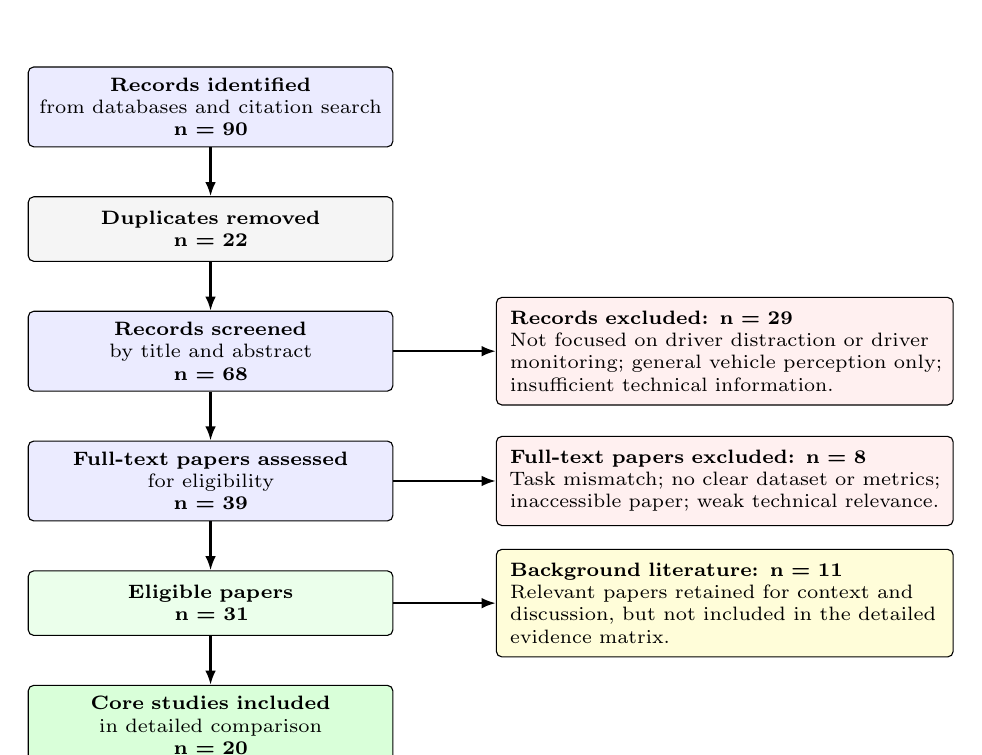
\begin{tikzpicture}[
    node distance=0.62cm,
    mainbox/.style={
        rectangle,
        draw=black,
        rounded corners=2pt,
        align=center,
        text width=4.35cm,
        minimum height=0.82cm,
        inner sep=4pt,
        font=\scriptsize
    },
    sidebox/.style={
        rectangle,
        draw=black,
        rounded corners=2pt,
        align=left,
        text width=5.45cm,
        inner sep=5pt,
        font=\scriptsize
    },
    arrow/.style={-{Latex[length=1.8mm]}, thick}
]

\node[mainbox, fill=blue!8] (id)
{\textbf{Records identified}\\from databases and citation search\\\textbf{n = 90}};

\node[mainbox, below=of id, fill=gray!8] (dup)
{\textbf{Duplicates removed}\\\textbf{n = 22}};

\node[mainbox, below=of dup, fill=blue!8] (screen)
{\textbf{Records screened}\\by title and abstract\\\textbf{n = 68}};

\node[mainbox, below=of screen, fill=blue!8] (full)
{\textbf{Full-text papers assessed}\\for eligibility\\\textbf{n = 39}};

\node[mainbox, below=of full, fill=green!8] (eligible)
{\textbf{Eligible papers}\\\textbf{n = 31}};

\node[mainbox, below=of eligible, fill=green!15] (final)
{\textbf{Core studies included}\\in detailed comparison\\\textbf{n = 20}};

\node[sidebox, right=1.30cm of screen, fill=red!6] (ex1)
{\textbf{Records excluded: n = 29}\\
Not focused on driver distraction or driver monitoring; general vehicle perception only; insufficient technical information.};

\node[sidebox, right=1.30cm of full, fill=red!6] (ex2)
{\textbf{Full-text papers excluded: n = 8}\\
Task mismatch; no clear dataset or metrics; inaccessible paper; weak technical relevance.};

\node[sidebox, right=1.30cm of eligible, fill=yellow!15] (ex3)
{\textbf{Background literature: n = 11}\\
Relevant papers retained for context and discussion, but not included in the detailed evidence matrix.};

\draw[arrow] (id) -- (dup);
\draw[arrow] (dup) -- (screen);
\draw[arrow] (screen) -- (full);
\draw[arrow] (full) -- (eligible);
\draw[arrow] (eligible) -- (final);

\draw[arrow] (screen.east) -- (ex1.west);
\draw[arrow] (full.east) -- (ex2.west);
\draw[arrow] (eligible.east) -- (ex3.west);

\end{tikzpicture}
}
\caption{PRISMA-style selection process used for the survey.}
\label{fig:prisma_corrected}
\end{figure}

\subsection{Reasons for Exclusion}

\begin{table}[H]
\centering
\caption{Full-text exclusion and background-use reasons.}
\label{tab:exclusion_reasons}
\small
\renewcommand{\arraystretch}{1.10}
\begin{tabularx}{0.92\linewidth}{>{\RaggedRight\arraybackslash}p{0.52\linewidth} c >{\RaggedRight\arraybackslash}X}
\toprule
\textbf{Reason} & \textbf{Number} & \textbf{Decision} \\
\midrule
Full text did not provide clear dataset, method or metric information. & 3 & Excluded after full-text assessment. \\
Task was too far from driver distraction or driver monitoring. & 2 & Excluded after full-text assessment. \\
Paper focused mainly on drowsiness/fatigue without useful distraction relevance. & 1 & Excluded after full-text assessment. \\
Paper was inaccessible or incomplete. & 1 & Excluded after full-text assessment. \\
Duplicate or highly similar technical contribution. & 1 & Excluded after full-text assessment. \\
Relevant but less central to the evidence matrix. & 11 & Retained for background discussion. \\
\bottomrule
\end{tabularx}
\normalsize
\end{table}

% =========================================================
\section{Research Landscape}

Driver distraction detection connects several research layers: distraction psychology, sensing modality, computer vision task, model family, dataset type, evaluation protocol and deployment platform. Confusion between these layers is one reason why the literature can appear more consistent than it actually is. For example, a ten-class image classifier trained on State Farm, a YOLO-based phone detector, a landmark-based drowsiness monitor and an IR-based night-time driver monitoring system are all relevant, but they do not solve the same task.

Figure~\ref{fig:landscape} summarises the landscape. The highlighted route is the main focus of this survey: RGB driver-distraction classification, low-light/IR/NIR data, domain adaptation and fair evaluation.

\begin{figure}[H]
\centering
\resizebox{0.98\linewidth}{!}{
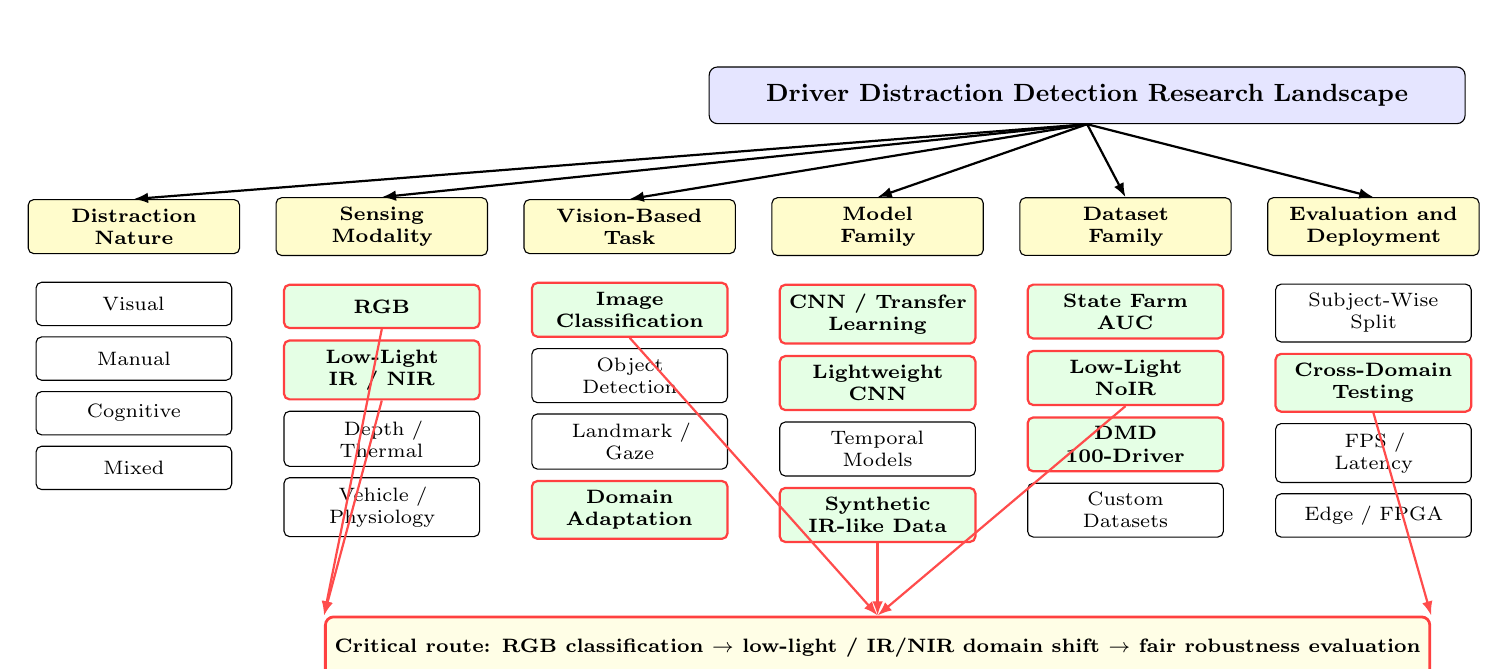
\begin{tikzpicture}[
    node distance=0.38cm and 0.50cm,
    root/.style={
        rectangle,
        rounded corners=3pt,
        draw=black,
        fill=blue!10,
        align=center,
        font=\small\bfseries,
        minimum width=9.6cm,
        minimum height=0.72cm
    },
    head/.style={
        rectangle,
        rounded corners=2pt,
        draw=black,
        fill=yellow!20,
        align=center,
        font=\scriptsize\bfseries,
        text width=2.45cm,
        minimum height=0.65cm
    },
    item/.style={
        rectangle,
        rounded corners=2pt,
        draw=black,
        align=center,
        font=\scriptsize,
        text width=2.25cm,
        minimum height=0.55cm
    },
    focus/.style={
        rectangle,
        rounded corners=2pt,
        draw=red!75,
        line width=0.8pt,
        fill=green!10,
        align=center,
        font=\scriptsize\bfseries,
        text width=2.25cm,
        minimum height=0.55cm
    },
    arrow/.style={-{Latex[length=1.8mm]}, thick}
]

\node[root] (root) {Driver Distraction Detection Research Landscape};

\node[head, below left=0.95cm and 5.95cm of root] (h1) {Distraction\\Nature};
\node[head, right=0.45cm of h1] (h2) {Sensing\\Modality};
\node[head, right=0.45cm of h2] (h3) {Vision-Based\\Task};
\node[head, right=0.45cm of h3] (h4) {Model\\Family};
\node[head, right=0.45cm of h4] (h5) {Dataset\\Family};
\node[head, right=0.45cm of h5] (h6) {Evaluation and\\Deployment};

\foreach \h in {h1,h2,h3,h4,h5,h6}{
    \draw[arrow] (root.south) -- (\h.north);
}

\node[item, below=0.35cm of h1] (v1) {Visual};
\node[item, below=0.13cm of v1] (v2) {Manual};
\node[item, below=0.13cm of v2] (v3) {Cognitive};
\node[item, below=0.13cm of v3] (v4) {Mixed};

\node[focus, below=0.35cm of h2] (s1) {RGB};
\node[focus, below=0.13cm of s1] (s2) {Low-Light\\IR / NIR};
\node[item, below=0.13cm of s2] (s3) {Depth /\\Thermal};
\node[item, below=0.13cm of s3] (s4) {Vehicle /\\Physiology};

\node[focus, below=0.35cm of h3] (t1) {Image\\Classification};
\node[item, below=0.13cm of t1] (t2) {Object\\Detection};
\node[item, below=0.13cm of t2] (t3) {Landmark /\\Gaze};
\node[focus, below=0.13cm of t3] (t4) {Domain\\Adaptation};

\node[focus, below=0.35cm of h4] (a1) {CNN / Transfer\\Learning};
\node[focus, below=0.13cm of a1] (a2) {Lightweight\\CNN};
\node[item, below=0.13cm of a2] (a3) {Temporal\\Models};
\node[focus, below=0.13cm of a3] (a4) {Synthetic\\IR-like Data};

\node[focus, below=0.35cm of h5] (d1) {State Farm\\AUC};
\node[focus, below=0.13cm of d1] (d2) {Low-Light\\NoIR};
\node[focus, below=0.13cm of d2] (d3) {DMD\\100-Driver};
\node[item, below=0.13cm of d3] (d4) {Custom\\Datasets};

\node[item, below=0.35cm of h6] (p1) {Subject-Wise\\Split};
\node[focus, below=0.13cm of p1] (p2) {Cross-Domain\\Testing};
\node[item, below=0.13cm of p2] (p3) {FPS /\\Latency};
\node[item, below=0.13cm of p3] (p4) {Edge / FPGA};

\node[
    rectangle,
    rounded corners=3pt,
    draw=red!75,
    fill=yellow!10,
    line width=1pt,
    below=0.92cm of a4,
    minimum width=12.4cm,
    minimum height=0.78cm,
    align=center,
    font=\scriptsize\bfseries
] (path) {Critical route: RGB classification \(\rightarrow\) low-light / IR/NIR domain shift \(\rightarrow\) fair robustness evaluation};

\draw[arrow, red!70] (s1.south) -- (path.north west);
\draw[arrow, red!70] (s2.south) -- (path.north west);
\draw[arrow, red!70] (t1.south) -- (path.north);
\draw[arrow, red!70] (a4.south) -- (path.north);
\draw[arrow, red!70] (d2.south) -- (path.north);
\draw[arrow, red!70] (p2.south) -- (path.north east);

\end{tikzpicture}
}
\caption{Research landscape of driver distraction detection, with emphasis on the link between RGB classification, low-light/IR/NIR domain shift and fair robustness evaluation.}
\label{fig:landscape}
\end{figure}

\begin{table}[H]
\centering
\caption{Survey taxonomy used to organise the literature.}
\label{tab:survey_taxonomy}
\small
\renewcommand{\arraystretch}{1.12}
\begin{tabularx}{\linewidth}{>{\RaggedRight\arraybackslash}p{0.22\linewidth} >{\RaggedRight\arraybackslash}p{0.36\linewidth} >{\RaggedRight\arraybackslash}X}
\toprule
\textbf{Layer} & \textbf{Branches} & \textbf{Why it matters} \\
\midrule
Distraction nature & Visual, manual, cognitive, mixed & Defines the behaviour being recognised. \\
Sensing modality & RGB, NoIR, IR/NIR, depth, thermal, vehicle signals & Determines whether the system can work across lighting conditions. \\
Task type & Image classification, detection, landmarks, temporal recognition, domain adaptation & Determines label type and whether results are comparable. \\
Dataset family & State Farm, AUC, LDDB, DAD, DMD, low-light NoIR, 100-Driver & Determines subject diversity, lighting range and generalisation risk. \\
Model family & CNN, lightweight CNN, CNN-ML, YOLO, LSTM/GRU, transformer, translation & Determines modelling strategy and computational burden. \\
Evaluation & Accuracy, macro-F1, per-class recall, confusion matrix, subject-wise split, cross-domain test & Determines whether reported performance is reliable. \\
Deployment & CPU, GPU, edge device, Raspberry Pi, Jetson, FPGA & Determines whether the method is only offline or practically deployable. \\
\bottomrule
\end{tabularx}
\normalsize
\end{table}

% =========================================================
\section{Datasets and Lighting Conditions}

Datasets are not neutral containers of images. In driver monitoring, the dataset often determines the apparent difficulty of the problem. The same model can look strong on a controlled RGB dataset and weak under different lighting, camera placement or driver population. This section therefore separates RGB classification datasets from low-light and IR/NIR datasets.

\subsection{RGB Image-Classification Datasets}

The State Farm Distracted Driver Detection dataset is widely used for image-level classification. It contains ten classes: safe driving, texting right, talking on the phone right, texting left, talking on the phone left, operating the radio, drinking, reaching behind, hair/makeup and talking to a passenger \parencite{kaggleStateFarm}. Its value is that the task is simple to formulate and easy to reproduce: one image, one label.

The weakness is that it does not represent all deployment conditions. It is not an object-detection dataset because it does not provide bounding boxes. It is also vulnerable to subject leakage if images are randomly split. If the same driver appears in training and testing, the model may learn identity, clothing, cabin background or camera position. For this reason, subject-wise splitting is more meaningful than random image splitting.

Other RGB datasets, including AUC, LDDB, DAD and custom datasets, provide additional benchmarks \parencite{eraqi2019driver,li2022,wu2024}. They differ in class labels, driver diversity, camera angle and evaluation protocol, so their reported metrics should not be treated as directly interchangeable.

\subsection{Low-Light, IR and NIR Datasets}

Low-light and IR/NIR studies are important because practical driver monitoring must work when visible light is poor. Table~\ref{tab:lowlight_datasets} compares the most relevant low-light and IR/NIR studies identified in this survey.

\begin{table}[H]
\centering
\caption{Low-light, IR/NIR and day-night datasets relevant to driver monitoring.}
\label{tab:lowlight_datasets}
\scriptsize
\renewcommand{\arraystretch}{1.14}
\setlength{\tabcolsep}{2.4pt}
\begin{adjustbox}{max width=\linewidth}
\begin{tabular}{
>{\RaggedRight\arraybackslash}p{2.8cm}
>{\RaggedRight\arraybackslash}p{1.0cm}
>{\RaggedRight\arraybackslash}p{2.6cm}
>{\RaggedRight\arraybackslash}p{3.1cm}
>{\RaggedRight\arraybackslash}p{2.4cm}
>{\RaggedRight\arraybackslash}p{3.3cm}}
\toprule
\textbf{Study / dataset} & \textbf{Year} & \textbf{Sensor / modality} & \textbf{Scale} & \textbf{Task relevance} & \textbf{Main caution} \\
\midrule
Saad et al. low-light dataset & 2020 & Raspberry Pi NoIR camera with IR LEDs & 70 drivers, 5 car models, 52,350 frames, 10 classes & Direct low-light driver distraction recognition & Split protocol and cross-domain transfer need careful checking. \\
Mendeley low-light dataset & 2020 & NoIR low-light support & Dataset associated with Saad et al. & Useful for night-time recognition & Should not be treated as equivalent to real NIR fleet data. \\
Shen and Lin & 2023 & Visible and infrared images & Day/night visible-infrared translation study & Directly relevant to RGB-IR domain shift & Synthetic translation is not physical IR recovery. \\
DMD / VicomTECH & 2020 & RGB, depth, IR videos & 41 hours, 37 drivers, 3 camera views & Multimodal driver monitoring and distraction activities & Broader than distraction classification only. \\
100-Driver & 2023 & Daytime RGB and night-time NIR & 100 drivers, 470,208 images, 4 views, 5 vehicles & Strong day/night and cross-camera evidence & Task categories differ from State Farm. \\
InSight & 2020 & NIR LED-based low-light setup & 15 drivers, controlled and real-road low-light settings & Low-light driver state monitoring & Not a full 10-class distraction dataset. \\
IR driver monitoring & 2023 & Infrared video & Real-time driver monitoring & Supports night-time in-cabin monitoring & Focuses more on drowsiness/head pose than distraction. \\
RGBDT activity recognition & 2024 & RGB, depth and thermal infrared & Multimodal activity recognition & Useful for lighting-robust activity recognition & Sensor setup differs from normal RGB cameras. \\
\bottomrule
\end{tabular}
\end{adjustbox}
\normalsize
\end{table}

Saad et al. are useful because the study directly addresses low-light driver distraction recognition and reports a best accuracy of 95.48\% using Convolutional GRU \parencite{saad2020lowlight}. The result is important, but it should not be read as proof that low-light distraction recognition is solved. A stronger interpretation is that NoIR-supported low-light data can support high within-dataset performance, while the harder question is whether models trained under one lighting and camera setup generalise to different drivers, vehicles, cameras and night-time domains.

DMD/VicomTECH and 100-Driver broaden the discussion. DMD provides RGB, depth and IR data from multiple in-cabin cameras and includes distraction-related activities \parencite{ortega2020dmd}. The 100-Driver dataset adds a larger driver population and includes daytime RGB and night-time NIR modalities \parencite{wang2023hundreddriver}. These datasets suggest that the next useful step for the field is not another RGB-only accuracy comparison, but controlled testing across lighting and sensor domains.

\subsection{What the Dataset Evidence Shows}

Table~\ref{tab:dataset_evidence} summarises the dataset evidence more directly. The table is not intended to rank datasets; it shows which kinds of evidence are available and which are still missing.

\begin{table}[H]
\centering
\caption{Dataset evidence for lighting-robust driver distraction recognition.}
\label{tab:dataset_evidence}
\small
\renewcommand{\arraystretch}{1.12}
\begin{tabularx}{\linewidth}{
>{\RaggedRight\arraybackslash}p{0.22\linewidth}
>{\RaggedRight\arraybackslash}p{0.14\linewidth}
>{\RaggedRight\arraybackslash}p{0.14\linewidth}
>{\RaggedRight\arraybackslash}p{0.14\linewidth}
>{\RaggedRight\arraybackslash}X}
\toprule
\textbf{Dataset family} & \textbf{RGB} & \textbf{Low-light / IR} & \textbf{Driver diversity} & \textbf{Main value for this survey} \\
\midrule
State Farm-style datasets & Strong & Weak & Moderate & Useful baseline for image classification, but limited lighting robustness evidence. \\
AUC / posture datasets & Strong & Limited & Moderate & Useful for posture and distraction classification comparisons. \\
Low-light NoIR dataset & Limited RGB comparison & Strong & 70 drivers & Directly relevant to low-light distraction recognition. \\
DMD / VicomTECH & Strong & Strong & 37 drivers & Useful multimodal evidence across RGB, depth and IR. \\
100-Driver & Strong & Strong NIR & 100 drivers & Strong evidence for day/night and cross-view evaluation. \\
Custom real-time datasets & Variable & Variable & Often small & Useful for deployment examples, but reproducibility is often weaker. \\
\bottomrule
\end{tabularx}
\normalsize
\end{table}

% =========================================================
\section{Algorithm Families}

The reviewed studies use several model families. The important point is not simply which model reports the highest accuracy, but whether the model is evaluated under a fair and realistic protocol.

\focuspara{Handcrafted features and traditional machine learning}
Earlier methods used HOG, SIFT, contour descriptors, skin segmentation or gaze-related features with SVM or random forest classifiers \parencite{hssayeni2017,zhao2012postures}. These methods are easier to interpret but depend heavily on manually designed features.

\focuspara{CNN image classification}
CNN-based classification remains the natural baseline for image-level datasets such as State Farm. ResNet, VGG, EfficientNet, MobileNet, Swin Transformer and custom CNNs have all been used for driver behaviour classification \parencite{huang2020,li2022,khan2023,zhang2024}. The risk is that CNNs can learn dataset-specific cues if the split protocol is weak.

\focuspara{Lightweight CNNs}
Lightweight models are important for practical deployment because in-cabin systems may need to run on limited hardware. MobileNet-style models and compact architectures are therefore useful, but they should be evaluated using model size, FPS and latency, not only accuracy \parencite{wu2024,wang2022}.

\focuspara{Hybrid CNN-machine learning pipelines}
Some studies use CNNs for feature extraction and then apply PCA, SVM or other classifiers \parencite{revathi2025,alkinani2022}. This can be useful for dimensionality reduction and controlled comparison, but it does not remove the need for subject-wise testing.

\focuspara{Object detection}
YOLO, Faster R-CNN and EfficientDet are relevant when the target is to localise phones, hands or objects \parencite{sajid2021,kanimozhi2025,elshamy2024}. These methods should not be directly compared with image classification unless the dataset contains compatible bounding-box annotations.

\focuspara{Temporal models}
Driver behaviour is often temporal. A single image may not capture the difference between reaching, turning, checking a mirror or preparing to interact with a device. Saad et al. used temporal models such as ConvLSTM and ConvGRU on low-light data, with Convolutional GRU reporting the best result \parencite{saad2020lowlight}. This supports sequence modelling, especially when frame order is available.

\focuspara{Visible-infrared translation and synthetic IR-like generation}
Visible-infrared translation is relevant because daytime RGB and night-time IR/NIR belong to different domains \parencite{shen2023visible}. The wording must be precise: RGB images cannot be transformed into true physical IR images. A more defensible aim is to generate synthetic IR-like or NIR-style samples for augmentation and domain adaptation, then test whether they improve robustness on real low-light or IR/NIR data.

% =========================================================
\section{Deployment Evidence}

Deployment evidence is weaker than classification evidence. Many studies report accuracy but do not report latency, FPS, power, model size or hardware resource usage.

\focuspara{CPU and GPU}
GPU results are useful for training and offline evaluation, but they do not prove in-vehicle deployment. A model that performs well on a GPU may be too slow or power-hungry for an embedded platform.

\focuspara{Edge devices}
Raspberry Pi and Jetson-style platforms appear in several real-time monitoring studies \parencite{kurian2023,mantrala2025,hariharan2023edge}. These studies are useful because they move closer to deployment, but they often use smaller datasets or custom test settings.

\focuspara{FPGA}
FPGA work is relevant to low-latency and energy-efficient inference, but the evidence must be hardware-specific. A useful FPGA paper should report quantisation, throughput, latency, FPS, power, energy per frame, LUTs, DSPs, BRAM and accuracy loss after compression or mapping \parencite{heenetimulla2022}. Without these details, the hardware contribution is too vague.

% =========================================================
\clearpage
\section{Evidence Matrix of Core Studies}

The detailed comparison is divided into two readable tables. Table~\ref{tab:core_facts} gives the technical facts. Table~\ref{tab:core_value} gives the contribution and limitation.

\begingroup
\footnotesize
\setlength{\tabcolsep}{2.4pt}
\renewcommand{\arraystretch}{1.18}

\begin{longtable}{
>{\RaggedRight\arraybackslash}p{0.035\linewidth}
>{\RaggedRight\arraybackslash}p{0.155\linewidth}
>{\RaggedRight\arraybackslash}p{0.155\linewidth}
>{\RaggedRight\arraybackslash}p{0.145\linewidth}
>{\RaggedRight\arraybackslash}p{0.235\linewidth}
>{\RaggedRight\arraybackslash}p{0.145\linewidth}
}
\caption{Technical facts of the core studies.}
\label{tab:core_facts}\\

\toprule
\textbf{No.} &
\textbf{Authors / year} &
\textbf{Dataset} &
\textbf{Task type} &
\textbf{Method} &
\textbf{Metric} \\
\midrule
\endfirsthead

\toprule
\textbf{No.} &
\textbf{Authors / year} &
\textbf{Dataset} &
\textbf{Task type} &
\textbf{Method} &
\textbf{Metric} \\
\midrule
\endhead

\bottomrule
\endfoot

1 & Kashevnik et al. (2021) & Review-based & Survey & Literature review and framework & N/A \\
2 & Revathi et al. (2025) & State Farm & Image classification & CNN feature extraction, PCA, SVM & 99.3\% Acc.; 98.9\% macro-F1 \\
3 & Saad et al. (2020) & Low-light NoIR dataset & Image / sequence classification & VGG16, ResNet50V2, InceptionV3, MobileNetV2, ConvLSTM, ConvGRU & 95.48\% Acc. \\
4 & Shen and Lin (2023) & Visible and infrared driver data & Day/night recognition & Visible-infrared translation and recognition & Reported \\
5 & Ortega et al. (2020) & DMD / VicomTECH & Driver monitoring & RGB-depth-IR multimodal dataset & N/A \\
6 & Wang et al. (2023) & 100-Driver & Driver distraction classification & RGB/NIR, cross-camera and cross-vehicle evaluation & Reported \\
7 & Mantrala et al. (2025) & Mixed video/image sources & Hybrid detection & MediaPipe, YOLOv5, MobileNetV3, rules & 88.1\% Acc.; 0.86 F1 \\
8 & R. K. and Mathew (2024) & State Farm & Image classification & ReLU-BiLSTM with attention & 95.87\% Acc.; 95.24\% F1 \\
9 & Kanimozhi et al. (2025) & Distracted-driver data & Object detection / classification & YOLO and CNN & 88-92\% reported \\
10 & Heenetimulla et al. (2022) & Driver posture and heart-rate data & Mobile-use detection and health monitoring & FPGA, camera, smartwatch & 93.49\% mobile-use detection \\
11 & Wei et al. (2022) & AUC dataset & Image classification & ResNet-50 & 43.5\% ten-class; 77.9\% binary \\
12 & Kurian and Soori (2023) & Real-time camera data & Drowsiness / distraction monitoring & Haar, Dlib, EAR, MAR, gaze tracking & 94.1\% drowsiness; 89\% distraction \\
13 & Wu et al. (2024) & DAD dataset & Distraction recognition & DDDNet, MobileNetV2, contrastive learning & 87.12\% Acc.; 0.9009 AUC \\
14 & Abouelnaga et al. (2018) & AUC & Posture classification & CNN ensemble & 95.98\% Acc. \\
15 & Hssayeni et al. (2017) & Distracted-driver images & Classification & Handcrafted features vs. deep learning & Not reported \\
16 & Huang et al. (2020) & State Farm & Image classification & Hybrid CNN framework & Reported \\
17 & Li et al. (2022) & LDDB and State Farm & Image classification & Octave-like CNN & Reported \\
18 & Sajid et al. (2021) & State Farm & Detection-style framework & EfficientDet, Faster R-CNN, YOLOv3 & Reported \\
19 & Khan et al. (2023) & State Farm / AUC & Image classification & EfficientNet with channel attention & 99.58\% reported \\
20 & Zhang et al. (2024) & AUC-DD / State Farm & Image classification & Swin Transformer & 99.71\% reported \\

\end{longtable}
\endgroup

\begingroup
\footnotesize
\setlength{\tabcolsep}{2.8pt}
\renewcommand{\arraystretch}{1.18}

\begin{longtable}{
>{\RaggedRight\arraybackslash}p{0.035\linewidth}
>{\RaggedRight\arraybackslash}p{0.155\linewidth}
>{\RaggedRight\arraybackslash}p{0.360\linewidth}
>{\RaggedRight\arraybackslash}p{0.360\linewidth}
}
\caption{Main contribution and limitation of the core studies.}
\label{tab:core_value}\\

\toprule
\textbf{No.} &
\textbf{Study} &
\textbf{Main contribution} &
\textbf{Main limitation / caution} \\
\midrule
\endfirsthead

\toprule
\textbf{No.} &
\textbf{Study} &
\textbf{Main contribution} &
\textbf{Main limitation / caution} \\
\midrule
\endhead

\bottomrule
\endfoot

1 & Kashevnik et al. (2021) & Provides a useful taxonomy and framework for driver distraction detection methods. & Review paper; does not evaluate a new model. \\
2 & Revathi et al. (2025) & Strong State Farm result with accuracy and macro-F1. & High result still depends on split protocol and subject independence. \\
3 & Saad et al. (2020) & Direct low-light driver distraction recognition using NoIR-supported data. & Needs careful interpretation of driver/session independence and cross-domain transfer. \\
4 & Shen and Lin (2023) & Links daytime visible and night-time infrared domains. & Translation output should not be treated as true physical IR. \\
5 & Ortega et al. (2020) & Provides broad RGB-depth-IR driver monitoring data. & Wider than distraction classification alone. \\
6 & Wang et al. (2023) & Provides large-scale day/night RGB/NIR driver data. & Task labels differ from State-Farm-style classification. \\
7 & Mantrala et al. (2025) & Demonstrates an edge-AI style pipeline. & Mixed sources make direct benchmarking difficult. \\
8 & R. K. and Mathew (2024) & Shows a lightweight temporal-style model on State Farm. & Needs stronger unseen-driver and deployment evidence. \\
9 & Kanimozhi et al. (2025) & Represents object-detection-based distraction work. & Detection and classification results are not directly comparable. \\
10 & Heenetimulla et al. (2022) & Gives a hardware-related FPGA example. & Task differs from ten-class driver distraction classification. \\
11 & Wei et al. (2022) & Shows binary safe/unsafe classification is easier than ten-class recognition. & Demonstrates difficulty of fine-grained classification. \\
12 & Kurian and Soori (2023) & Gives a real-time Raspberry Pi monitoring example. & Stronger on drowsiness than full distraction recognition. \\
13 & Wu et al. (2024) & Contributes lightweight/open-set recognition direction. & Dataset and task differ from State Farm. \\
14 & Abouelnaga et al. (2018) & Important benchmark for posture classification. & Older and more controlled than deployment settings. \\
15 & Hssayeni et al. (2017) & Motivates CNN features over handcrafted features. & Some metrics are not available in the current summary. \\
16 & Huang et al. (2020) & Provides State-Farm-based hybrid CNN comparison. & Exact split and generalisation protocol should be checked. \\
17 & Li et al. (2022) & Presents efficient CNN design for distraction detection. & Cross-dataset robustness needs careful interpretation. \\
18 & Sajid et al. (2021) & Useful detection-style comparison using modern detectors. & Annotation compatibility must be considered. \\
19 & Khan et al. (2023) & Reports strong EfficientNet-channel-attention performance. & High accuracy needs careful split-protocol checking. \\
20 & Zhang et al. (2024) & Represents transformer-based distracted-driver classification. & Computational cost may be higher than lightweight alternatives. \\

\end{longtable}
\endgroup

% =========================================================
\clearpage
\section{Critical Quantitative Synthesis}

A direct accuracy leaderboard is not appropriate for this topic. The studies use different datasets, lighting conditions, split protocols, metrics and task definitions. A 99\% result on a random split can be less convincing than a lower score under subject-wise or cross-dataset testing. For that reason, Table~\ref{tab:metric_context} interprets reported results together with evaluation context.

\begin{table}[H]
\centering
\caption{Reported performance values and interpretation context.}
\label{tab:metric_context}
\footnotesize
\renewcommand{\arraystretch}{1.15}
\begin{tabularx}{\linewidth}{
>{\RaggedRight\arraybackslash}p{0.17\linewidth}
>{\RaggedRight\arraybackslash}p{0.16\linewidth}
>{\RaggedRight\arraybackslash}p{0.16\linewidth}
>{\RaggedRight\arraybackslash}p{0.16\linewidth}
>{\RaggedRight\arraybackslash}X}
\toprule
\textbf{Study} & \textbf{Reported value} & \textbf{Dataset / domain} & \textbf{Evaluation concern} & \textbf{Interpretation} \\
\midrule
Revathi et al. & 99.3\% Acc.; 98.9\% F1 & State Farm RGB & Split details matter & Strong within-dataset result, but not proof of low-light robustness. \\
Saad et al. & 95.48\% Acc. & Low-light NoIR & Cross-domain generalisation unclear & Important low-light evidence, but should be tested against other domains. \\
Mantrala et al. & 88.1\% Acc.; 0.86 F1 & Mixed sources & Dataset mixing & Useful system-level evidence, but not a clean benchmark comparison. \\
Wei et al. & 43.5\% ten-class; 77.9\% binary & AUC & Task difficulty changes result & Shows binary detection is much easier than fine-grained classification. \\
Wu et al. & 87.12\% Acc.; 0.9009 AUC & DAD & Different task setting & Useful lightweight evidence, but not directly comparable with State Farm. \\
Khan et al. & 99.58\% reported & State Farm / AUC & Split and leakage risk & High result should be interpreted through protocol details. \\
Zhang et al. & 99.71\% reported & AUC-DD / State Farm & Computational cost and split protocol & Transformer result is strong, but deployment and fairness need checking. \\
\bottomrule
\end{tabularx}
\normalsize
\end{table}

\begin{table}[H]
\centering
\caption{Evidence strength across major evaluation requirements. A tick means the study direction directly supports the evidence type; a dash means weak, indirect or not clearly reported evidence.}
\label{tab:evidence_strength}
\small
\renewcommand{\arraystretch}{1.16}
\begin{tabularx}{\linewidth}{
>{\RaggedRight\arraybackslash}p{0.22\linewidth}
c c c c c >{\RaggedRight\arraybackslash}X}
\toprule
\textbf{Study group} & \textbf{RGB} & \textbf{Low-light} & \textbf{IR/NIR} & \textbf{Subject split} & \textbf{Deployment} & \textbf{Main reading} \\
\midrule
State Farm CNN studies & \checkmark & -- & -- & Mixed & -- & Strong for RGB classification, weaker for lighting robustness. \\
Low-light NoIR study & -- & \checkmark & \checkmark & Needs checking & -- & Key evidence for low-light distraction recognition. \\
DMD / 100-Driver studies & \checkmark & \checkmark & \checkmark & Stronger & Mixed & Best evidence for modality and lighting diversity. \\
YOLO / object detection studies & \checkmark & Mixed & Mixed & Mixed & Mixed & Useful for localisation, but annotation type differs. \\
Edge / FPGA studies & Mixed & Mixed & Mixed & Often weak & \checkmark & Useful for deployment, but not always strong in dataset evaluation. \\
\bottomrule
\end{tabularx}
\normalsize
\end{table}

The main message from these tables is that high reported accuracy is not enough. The more useful question is whether the study tests the model under a realistic source of variation: unseen drivers, different lighting, different camera views, or a different dataset.

% =========================================================
\section{Key Trends}

Three trends are clear from the reviewed literature.

First, RGB image classification remains the easiest entry point into driver distraction detection. Datasets such as State Farm allow clean training and evaluation and CNN-based methods can achieve high reported accuracy. The weakness is that RGB benchmarks alone do not establish robustness.

Second, low-light and IR/NIR driver monitoring is becoming more important. Saad et al., DMD/VicomTECH and 100-Driver show that the literature is moving towards NoIR, IR, NIR and multimodal data \parencite{saad2020lowlight,ortega2020dmd,wang2023hundreddriver}. This gives the field a stronger direction than repeating RGB-only comparisons.

Third, many papers still report incomplete evidence. Accuracy is commonly reported, but subject-wise splits, cross-dataset testing, false-negative analysis, model size, latency and FPS are less consistent. This matters because a driver monitoring system must generalise, not only classify a familiar benchmark.

% =========================================================
\section{Open Challenges}

\focuspara{Lighting robustness}
A reliable in-cabin system must work across daylight, night-time, shadow, tunnel and artificial illumination. The field still lacks enough studies that train on one lighting domain and test on another.

\focuspara{Subject leakage}
If the same driver appears in both training and test sets, results can be inflated. Subject-wise splits are essential where subject labels are available.

\focuspara{Dataset bias}
Datasets differ in camera position, vehicle interior, driver demographics, lighting, class labels and annotation style. Cross-dataset testing is needed to reveal whether a model has learned behaviour or dataset-specific appearance.

\focuspara{Task mismatch}
Image classification and object detection are different problems. Image classification uses image-level labels, while detection requires bounding boxes. They should not be compared as if they used the same evidence.

\focuspara{Synthetic IR-like data}
Synthetic IR-like or NIR-style augmentation is promising, but the claim must be limited. It can support robustness testing and domain adaptation, but it does not recreate the physical information captured by a real IR sensor.

\focuspara{Deployment evidence}
Deployment claims should include latency, FPS, memory, power, model size and hardware resource usage. Without these metrics, a method remains mainly an offline model.

% =========================================================
\section{Future Research Direction}

The most useful next research direction is not another general comparison of CNNs on RGB images. A stronger direction is a controlled study of lighting-domain robustness in driver distraction detection.

A practical experimental design would compare:

\begin{enumerate}
    \item RGB-only training and RGB testing.
    \item RGB training with conventional augmentation.
    \item RGB training with synthetic IR-like or NIR-style augmentation.
    \item Testing on subject-wise RGB splits.
    \item Testing on real low-light, NoIR, IR or NIR data where available.
    \item Reporting accuracy, macro-F1, per-class recall, false negatives and confusion matrices.
\end{enumerate}

The key comparison is not simply whether synthetic IR-like images improve average accuracy. The more important question is whether they reduce failure under lighting shift and whether they improve difficult distraction classes without increasing false negatives in safety-critical cases.

Hardware acceleration can be treated as a second direction after the AI pipeline is stable. A convincing hardware study should report model compression, quantisation, latency, throughput, FPS, energy per frame, power, LUT usage, DSP usage, BRAM usage and accuracy loss after hardware mapping.

% =========================================================
\section{Threats to Validity}

This survey has limitations. Some industrial driver monitoring datasets and systems are not publicly accessible. Several papers report results without full details of split protocol or deployment hardware. Low-light and IR/NIR studies do not always use the same task definition as State-Farm-style image classification. Reported performance values are therefore interpreted as evidence within context, not as a universal ranking.

% =========================================================
\section{Conclusion}

This survey reviewed driver distraction detection with a focus on the transition from RGB image classification to low-light and IR/NIR robustness. The review shows that the field has many strong classification models, but less convincing evidence of robustness under lighting shift, unseen drivers and different sensor domains. RGB benchmarks such as State Farm remain useful, but they should not be treated as sufficient evidence for practical driver monitoring.

The main research opportunity is lighting-robust driver distraction recognition. Future work should combine RGB, low-light and IR/NIR evidence with subject-wise testing, cross-domain evaluation and class-level error analysis. Synthetic IR-like or NIR-style augmentation is a promising direction if it is framed carefully as domain adaptation rather than true IR recovery. Deployment and FPGA acceleration are also valuable, but they require separate hardware-specific evidence.

\nocite{young2003,dong2011,sahayadhas2012,sikander2019,ramzan2019,kaplan2015,doshi2009,vicente2015,horgan2021,dontoh2025modalities,dontoh2025visual,erso2022distraction,barr2005,saad2020dataset,dmdwebsite,kidu2024rgbdt,majdi2020drivenet,tan2020lrcn,streiffer2017dar,du2018multimodal,driverMHG2020,syndd2022,roma2022,hossain2022,gumaei2020}

\clearpage
\printbibliography[title={References}]

\end{document}

